\documentclass{article}
\title{Singular Value Decomposition for Image Compression}
\author{James DeGruccio}

\usepackage{hyperref}
\hypersetup{}

\usepackage{indentfirst}

\usepackage{graphicx}
\graphicspath{{./media/}}

\begin{document}
\maketitle

\section*{Introduction}

Singular Value Decomposition (SVD) is the factorization of any $m$$\times$$n$ matrix, $A$, into $U$$\Sigma$$V^T$. 
In this factorization, $\Sigma$ is a diagonal $m$$\times$$n$ matrix composed of the eigenvalues shared between $A$$A^T$ and $A^T$$A$.
$U$ and $V$ are $m$$\times$$m$ and $n$$\times$$n$ orthogonal matrices used with $\Sigma$ to produce $A = U \Sigma V^T$.

The matrix, $A$, can also be factored into a Compact/Reduced SVD\textsuperscript{\cite{compsvd}}.
The Compact/Reduced SVD shrinks size of the $\Sigma$ matrix by truncating the zero rows and columns in the $\Sigma$ matrix. 
The corresponding columns of $U$ and rows of $V$ are also removed, reducing the amount of data needed to store the Decomposition.
Formally, the Compact/Reduced SVD is denoted as $A = U_r \Sigma _r V_r^T$, where $r$ is the rank of matrix $A$, $U_r$ is $m$$\times$$r$, $V_r$ is $n$$\times$$r$, and $\Sigma_r$ is $r$$\times$$r$.
If $r \leq m, n$, the Compact SVD could losslessly store a matrix with less space compared to the raw matrix itself. 

A Truncated SVD\textsuperscript{\cite{compsvd}} can compress a matrix further by removing information from the matrix. 
This compression involves removing non-zero entries in $\Sigma$ and the corresponding columns of $U$ and rows of $V$. 

Since an image can be represented by a matrix of pixel values, an image can be factorized using Singular Value Decomposition.
The factored SVD matrix can then be truncated to implement a lossy compression algorithm. 

\begin{figure}[h]
    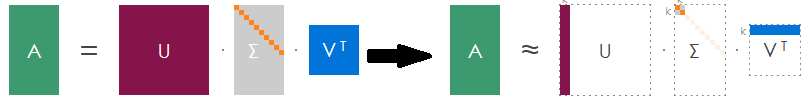
\includegraphics{Truncated-SVD.png}
    \centering
    \caption{Truncated SVD Illustration\textsuperscript{\cite{tsvd}}}
\end{figure}

\newpage
\section*{Method}

A Python program was written to implement the SVD compression algorithm. 
The program takes two command line arguements: 
\begin{enumerate}
    \item Input file name
    \item Size of truncated $\Sigma$ array. 
\end{enumerate}

To perform image compression, the Pillow Python library is used to read image files and NumPy is used to perform the Singular Value Decomposition. 
The $A$, $U$, $\Sigma$, $V$ matrices are organized in a class named \emph{SVD\_factored}.
This class has two methods, \emph{SVD\_Compact} and \emph{SVD\_Truncate}, which calculates the Compact SVD and Truncated SVD respectively. 
NumPy generates $U$, $\Sigma$, and $V$ matrices that are sorted from greatest to least with respect to $\Sigma$'s singular values.
This makes the Compact SVD and Truncate SVD algorithms incredibly simple, since all there is to do is truncate the last rows/columns of the matrices.
For Compact SVD, keep the first $r$ vectors.
For Truncate SVD, keep the first $n$ vectors, where $n$ is specified in command line arguements. 

\section*{Results}

Since I did give myself time to create a image file format for the SVD compression, there isn't a way to directly compare the actual compression ratios resulting from this algorithm.
Tim Baumann has a general formula on his website to calculate the compression ratio \cite{tsvd}. 
If $w$ is the image width, $h$ is the image height, and $n$ is truncated size of the singular values, the compression ratio is given below: \\

$ \frac{w \times h}{w \times n + n + n \times h} $ \\

I performed the SVD compression algorithm on a picture of my parent's dog. 
The results of this for various values of n can be seen below the references section.

\begin{figure}[h]
    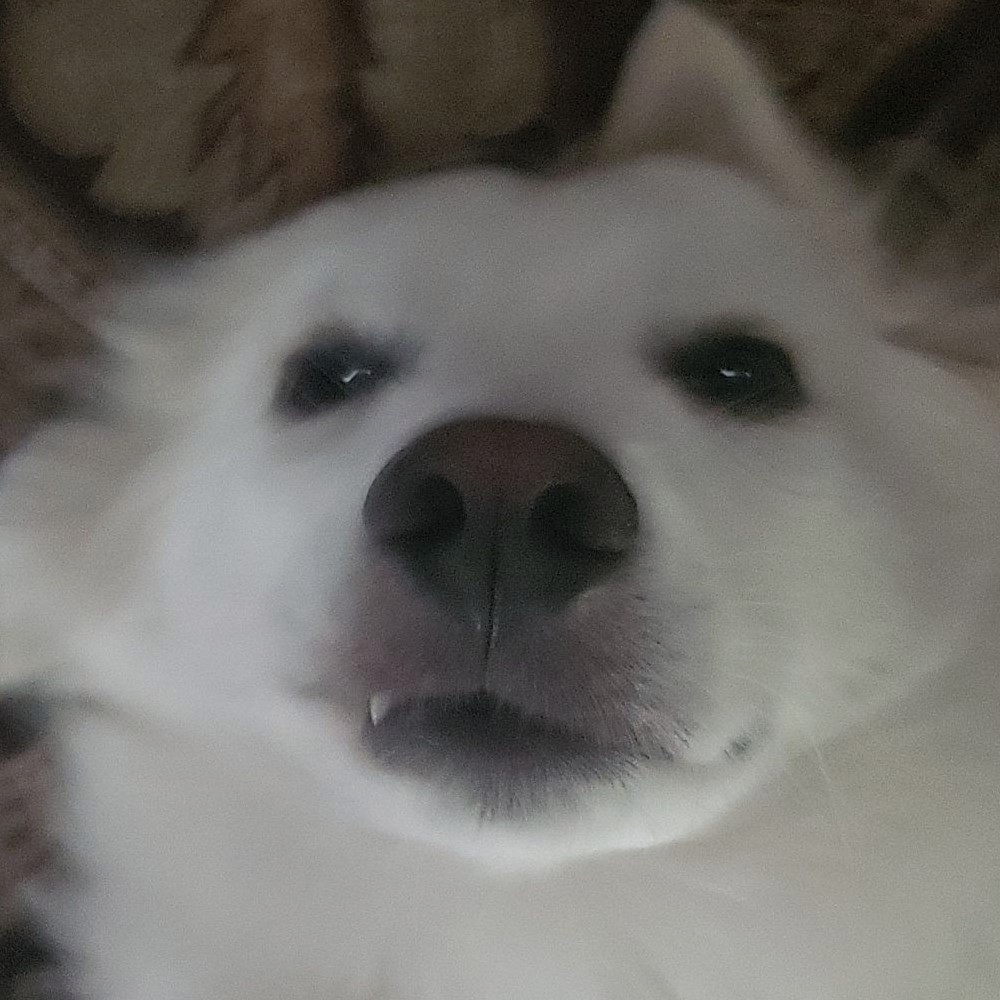
\includegraphics[scale=0.15]{lokip.jpg_svdc.png}
    \centering
    \caption{Original picture of Loki. }
\end{figure}

\begin{figure}[h]
    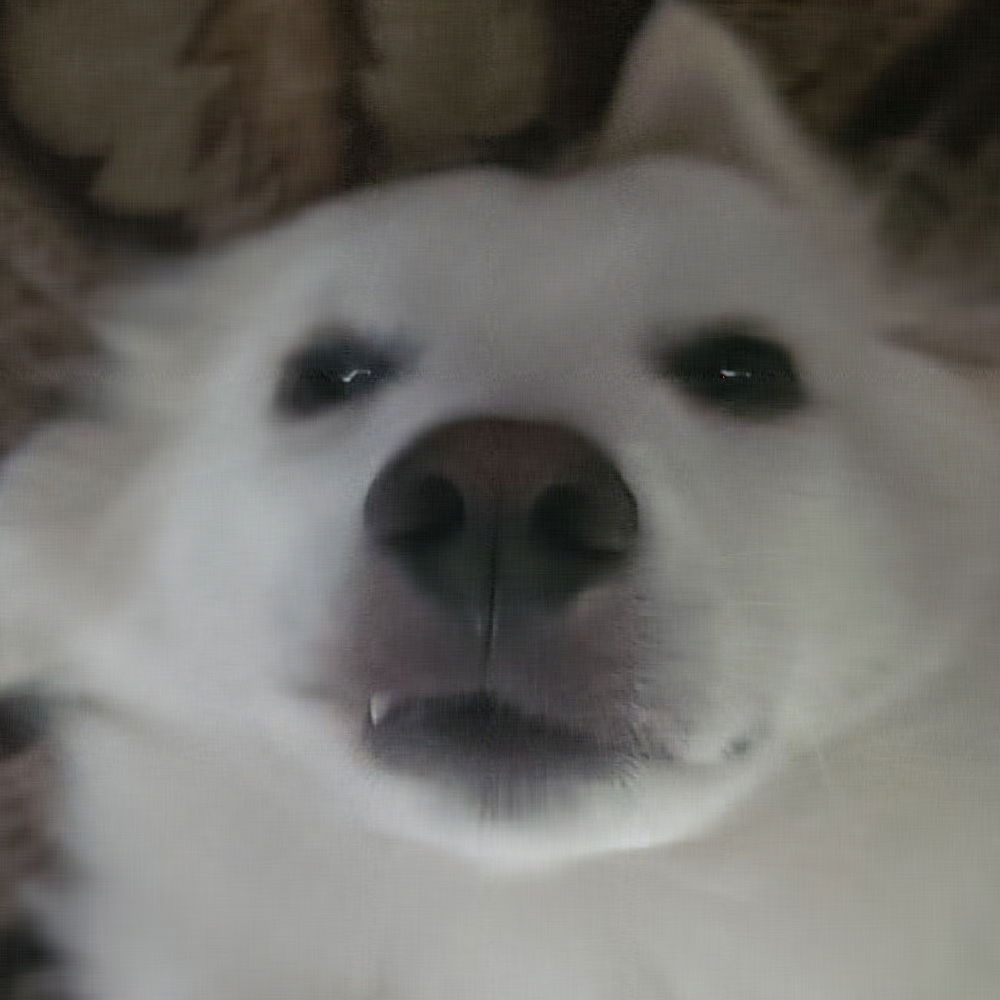
\includegraphics[scale=0.15]{lokip.jpg_svdt50.png}
    \centering
    \caption{Compressed with n=50}
\end{figure}

\begin{figure}[h]
    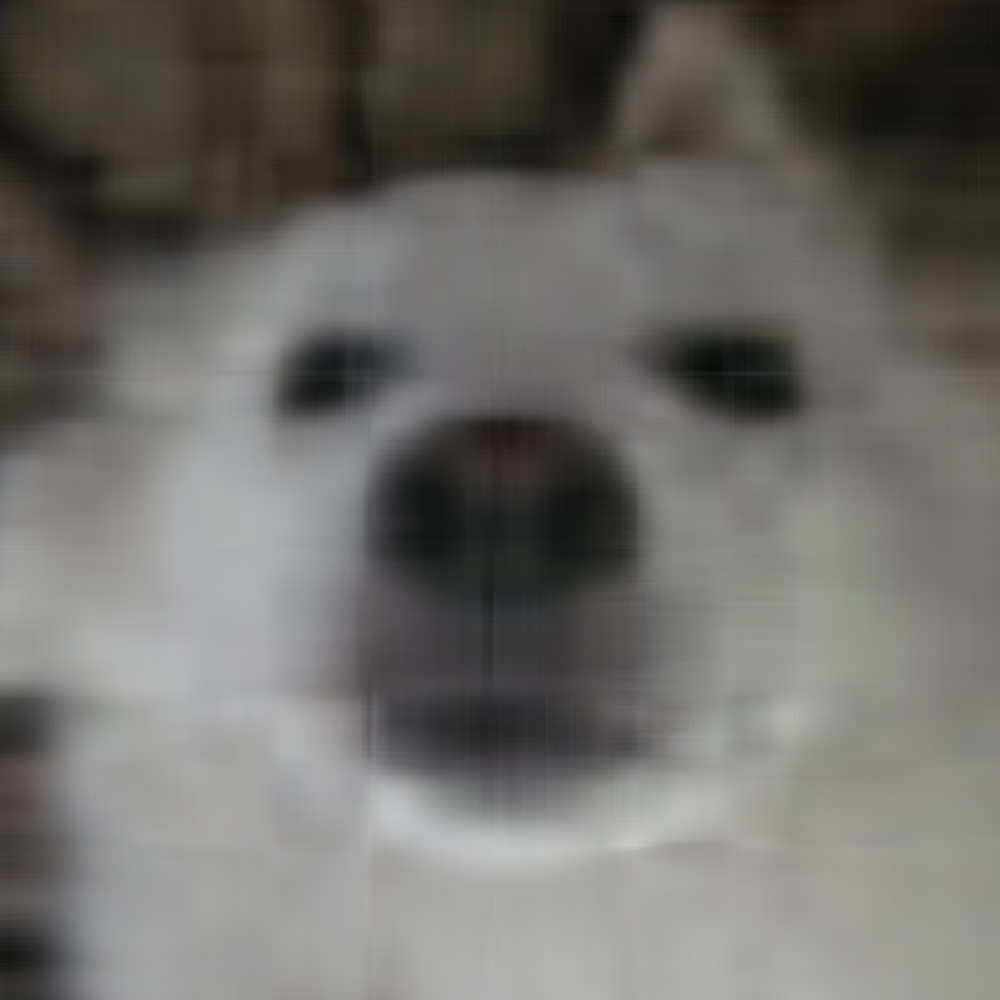
\includegraphics[scale=0.15]{lokip.jpg_svdt10.png}
    \centering
    \caption{Compressed with n=10}
\end{figure}

\begin{figure}[h]
    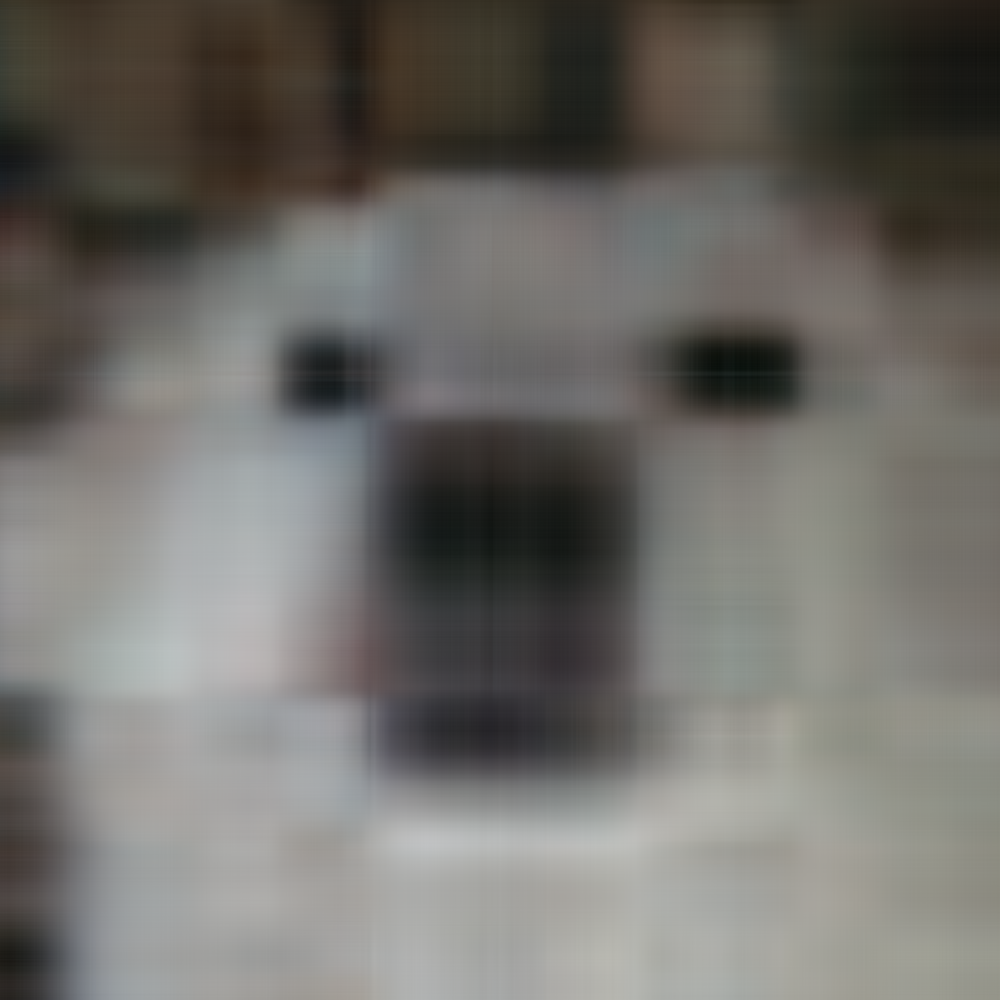
\includegraphics[scale=0.15]{lokip.jpg_svdt5.png}
    \centering
    \caption{Compressed with n=5}
\end{figure}

\begin{figure}[h]
    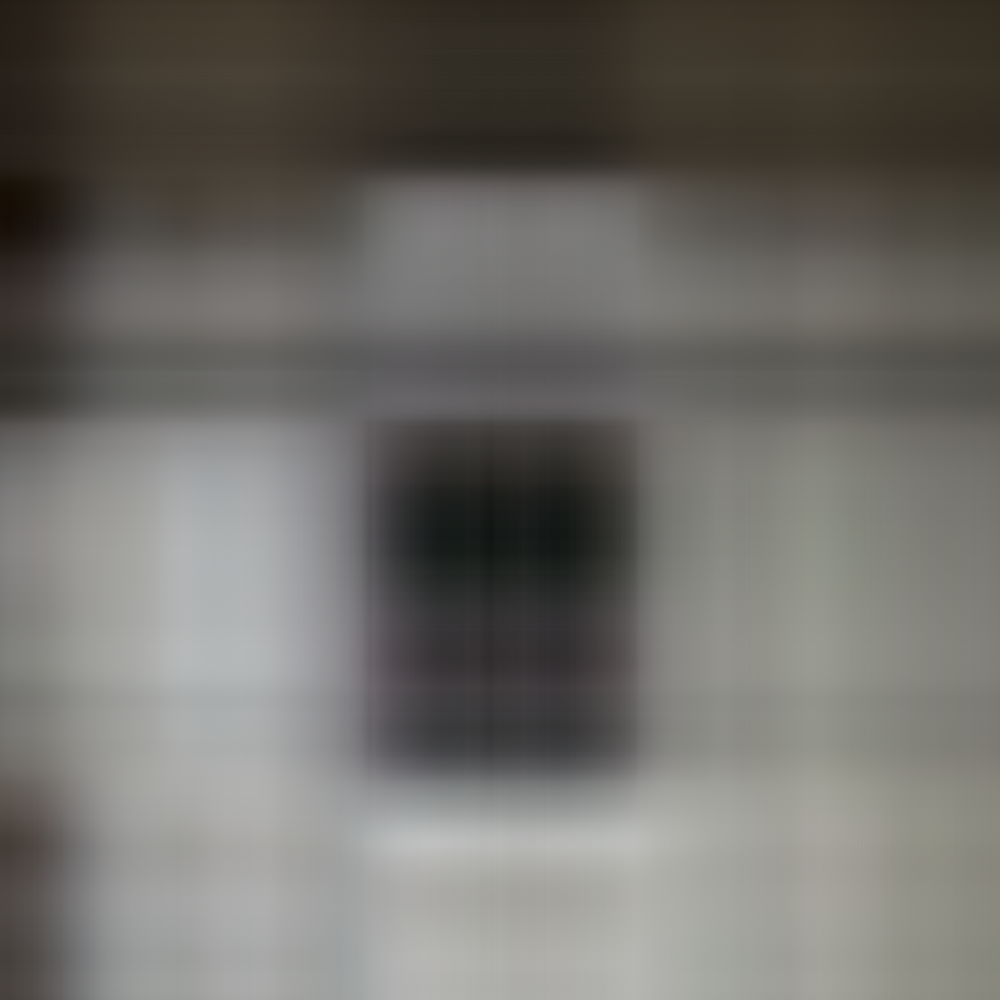
\includegraphics[scale=0.15]{lokip.jpg_svdt2.png}
    \centering
    \caption{Compressed with n=2}
\end{figure}

\begin{figure}[h]
    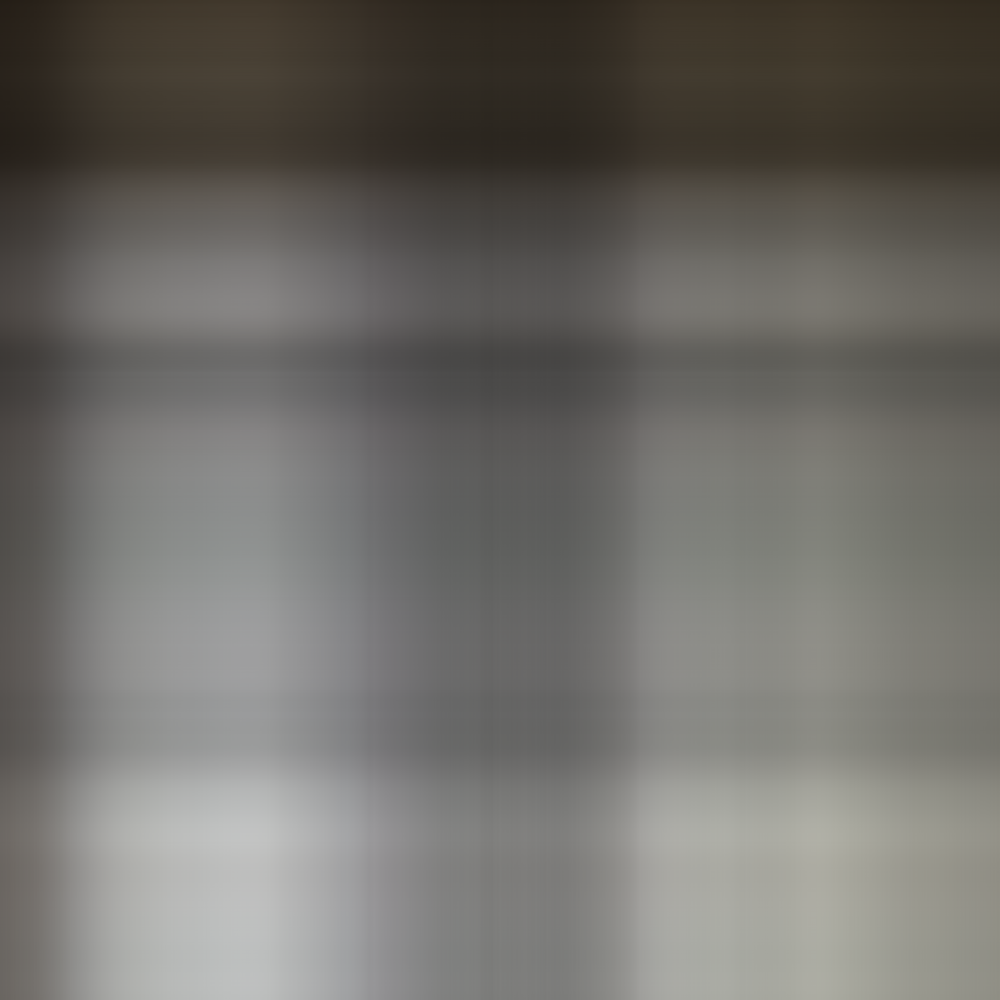
\includegraphics[scale=0.15]{lokip.jpg_svdt1.png}
    \centering
    \caption{Compressed with n=1}
\end{figure}

\begin{thebibliography}{}

    \bibitem{compsvd}
    Brigham Young University. (n.d.). The SVD and image compression. \url{https://acme.byu.edu/00000179-aa18-d402-af7f-abf806b60000/svd2020-pdf}

    \bibitem{tsvd}
    Baumann, T. (n.d.). Image compression with singular value decomposition. SVD-Demo: Image Compression. \url{https://timbaumann.info/svd-image-compression-demo/}

\end{thebibliography}

\end{document}